\chapter{Идентификация системы связанных релаксационных генераторов}

\newcommand{\RelaxBjtIi}{системы из трёх связанных релаксационных генераторов на паре комплиментарных транзисторов}
\newcommand{\RelaxShIi}{системы из трёх связанных релаксационных генераторов на основе триггеров Шмидта}

\section{Релаксационные генераторы: применение, модели}

Применение: собственно генераторы, источники питания.

Релаксационные генераторы, прямо или косвенно, получили широкое распространение
в схемотехнике. В первую очередь -- как собственно генераторы
сигналов, в первую очередь пилообразной формы~[??].
Некоторые подсистемы электрических схем, хоть и непосредственно
релаксационными генераторами, проявляют схожую динамику.
В первую очередь это импульсные системы питания, такие как
современные блоки питания электронной техники, DC/DC преобразователи.

Основными компонентами релаксационного генератора являются
времязадающая цепочка, чаще всего RC-цепочка,
и нелинейный (гистерезисный) переключающий элемент,
переключающий генератор из режима зарядки в режим разрядки и наоборот.
В качестве такого элемента может использоваться
динистор, газоразрядная лампа, триггер Шмидта,
другие электронные схемы.

\Cmt{Здесь условная схема}

Параметрами такого генератора являются
напряжения включения $V\Tidx{on}$ и выключения $V\Tidx{off}$
переключающего элемента,
напряжение питания $V\Tidx{cc}$,
ёмкость конденсатора $C$,
сопротивления цепей зарядки $R\Tidx{ch}$
и разрядки $R\Tidx{dis}$.
В данной работе, для лучшего проявления
хаотических режимов,
будем полагать, что времена зарядки и разрядки существенно отличаются.
Не снижая общности, считаем, что $R\Tidx{ch} \gg R\Tidx{dis} $.
При предварительном анализе можно считать $R\Tidx{dis} = 0$.
Тем не менее, для обеспечения корректности численного моделирования,
а также обеспечения адекватности модели требуется применение ненулевого значения $R\Tidx{dis}$.
Переменными состояния являются напряжение на конденсаторе $V\Tidx{c}$
и состояние переключающего элемента $On()$.
В случае использования нескольких релаксационных генераторов
эти величины будем обозначать соответственно как
$V_{i}$ и $ On_{i}()$.
При этом  $ On_{i}( V\Tidx{c}, \ldots )$ представляет собой
релейный гистерезисный элемент, обладающий памятью и задаётся алгоритмически.

\Cmt{Может быть рисунок релейного гистерезиса}

В этих условиях примем для определённости
(а в большинстве схемотехнических реализаций это так и есть),
что цепь зарядки включена постоянно, а цепь разрядки
включается при $V\Tidx{c} > V\Tidx{on} $ и выключается при
$V\Tidx{c} < V\Tidx{off}$.

С учётом этих обозначений модель релаксационного генератора
записывается следующим образом:
%
\begin{equation}
  C \od{V_c}{t}
  =
  \frac{V\Tidx{cc} - V\Tidx{c}}{R\Tidx{ch}}
  - \frac{V\Tidx{c}}{R\Tidx{dis}} \cdot On().
  \label{atu:eq:relax0}
\end{equation}

В случае одного релаксационного генератора
уравнение (\ref{atu:eq:relax0}) можно привести в безразмерному виду,
используя набор очевидных преобразований. В первую
очередь, величина $C R\Tidx{ch}$ определяет
постоянную времени процесса заряда, а процесс
разряда при условии $R\Tidx{ch} \gg R\Tidx{dis} $ будем считать происходящим практически мгновенно.
Далее, 

Если же применяется в одной схеме несколько релаксационных генераторов с различными параметрами,
то такое приведение практического смысла не имеет.


Элементная база, задачи. Почему возможны хаотические режимы



Не совсем прототип: Kennedy


\cite{mishenko_du_small_relax}

\section{Система из трёх связанных релаксационных генераторов на паре комплиментарных транзисторов}
\label{atu:sec:relax3d}


Исследуемый хаотический генератор представляет собой
систему из трёх релаксационных генераторов,
переключающий элемент в каждом из них реализован
на паре комплиментарных транзисторов~(рис.~\ref{atu:f:relax3d_schem}).

\begin{figure}[htb!]
  \centerline{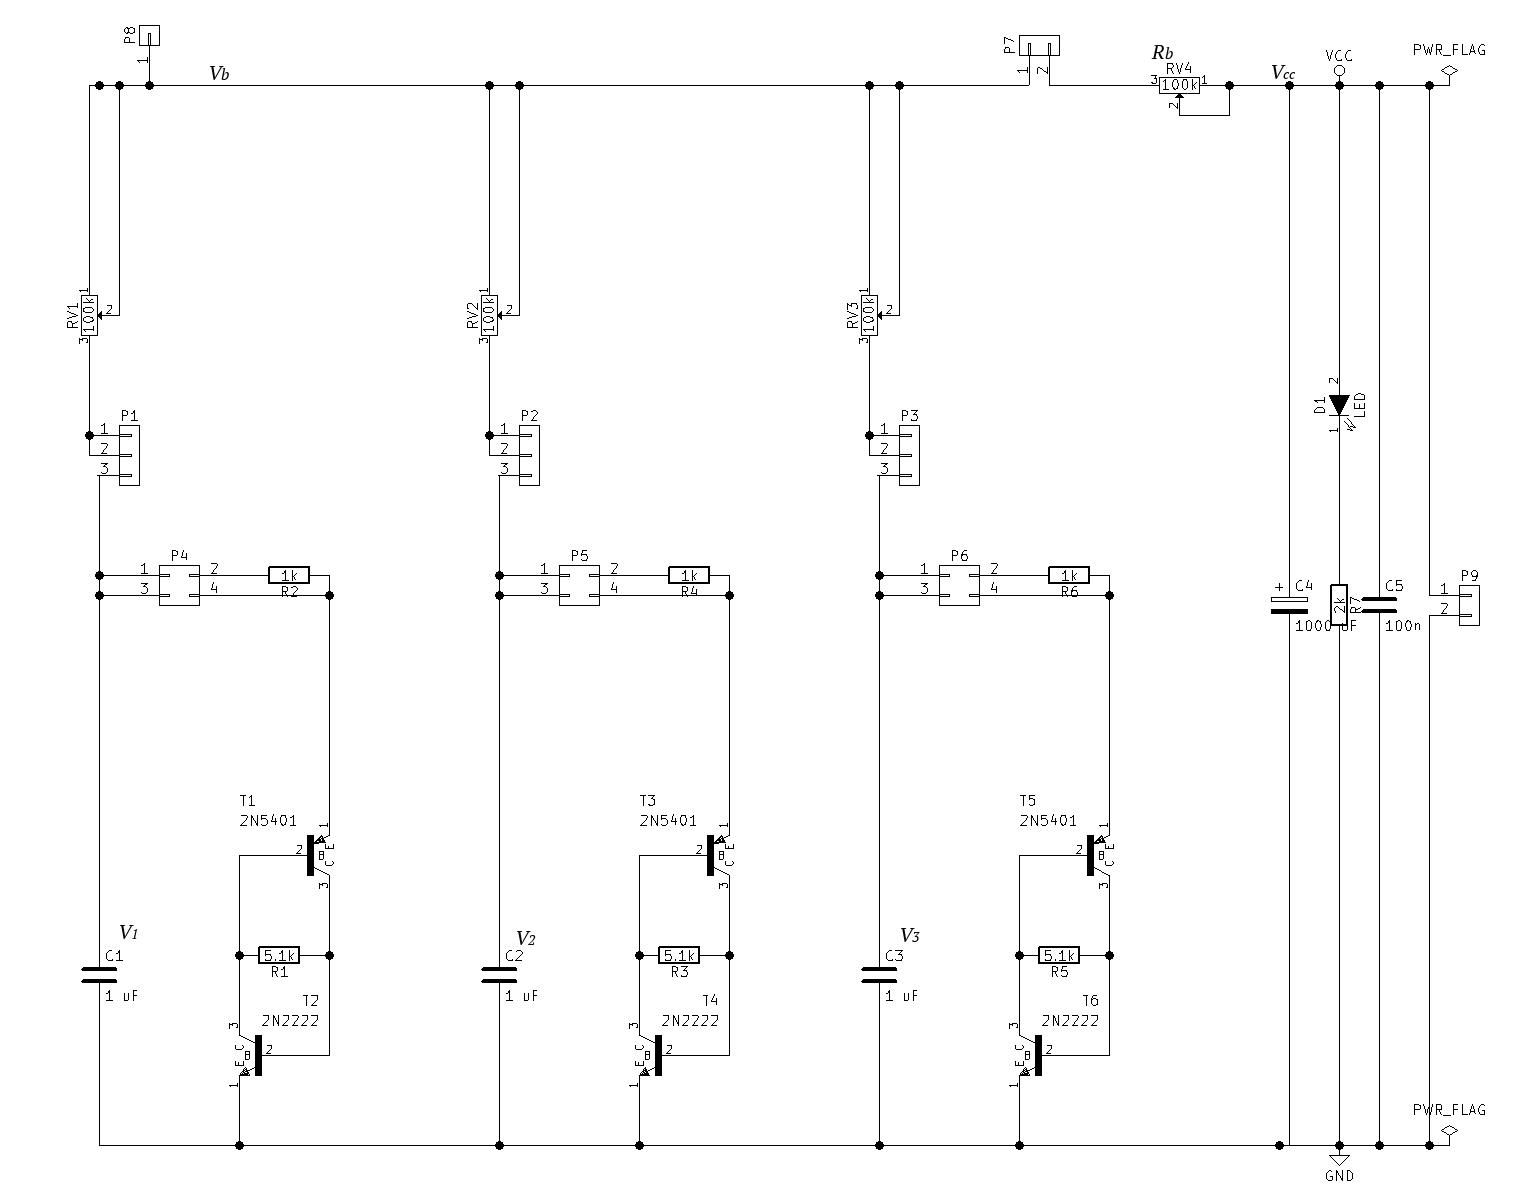
\includegraphics[width=0.8\textwidth]{p/relax3d_schem.png} }
  \caption{Электрическая схема \RelaxBjtIi}
  \label{atu:f:relax3d_schem}
\end{figure}

При создании данной схемы преследовались следующие задачи:
\begin{itemize}

  \item
    работоспособность схемы при малом напряжении питания $V\Tidx{cc}$,
    желательна возможность использования общего питания с микроконтроллером,
    при этом не требуются дополнительные согласующие элементы
    между генератором и АЦП микроконтроллера -- следовательно,
    меньше элементов, которые могут вносить искажения при измерении;

  \item
    относительно низкие рабочие частоты релаксационных генераторов --
    для уменьшения влияния индуктивностей и взаимных связей, не описываемых моделью,
    уменьшению шумов измерения, вызванных искажениями высокочастотных сигналов;

  \item
    возможность оперативно изменять параметры схемы, как отключая отдельные генераторы,
    так и вводя дополнительные элементы.

\end{itemize}

Возможность работы при низком напряжении питания в данной схеме обеспечивается
применением переключающего элемента с параметрами
$V\Tidx{on} \approx \SI{1.0}{\volt}$,
$V\Tidx{off} \approx \SI{0.6}{\volt}$.
При этом, напряжение питания $V\Tidx{cc} \approx \SI{3}{\volt}$
обеспечивает достаточный диапазон для изменения параметров генератора.
Любое из измеряемых напряжений $V_b$, $V_1$ -- $V_3$
заведомо не превосходит $V\Tidx{cc}$,
что позволяет использовать непосредственную связь
между элементами схемы и АЦП микроконтроллера.
Входные сопротивление каналов АЦП $R\Tidx{measure} \approx \SI{10e7}{\ohm}$
и ёмкость $C\Tidx{measure} \approx \SI{10}{\pico\farad} $
не вносят заметных искажений в работу генератора.

Относительно низкие (десятки и сотни Герц) рабочие частоты
релаксационных элементов были получены путём выбора соответствующих
ёмкостей:
$C_1$ -- $C_3 = \SI{1.0}{\micro\farad}$,
и сопротивлений:
$R_{v1}$ -- $R_{v3} = 1-\SI{100}{\kilo\ohm}$.
Каждое из указанных сопротивлений было подстроечным, для обеспечения
настройки параметров каждого из генераторов. Также подстроечным было сопротивление
$ R_{b} = 1-\SI{100}{\kilo\ohm}$.

Выбранные параметры генераторов определяют небольшой ток
потребления схемы, порядка единиц миллиампер, что
практически не оказывает влияния на работу
системы стабилизации напряжения питания микроконтроллера.
Тем не менее, импульсный характер энергопотребления
релаксационных генераторов может привести
к локальным возмущениям $V\Tidx{cc}$, что
как отрицательно сказывается на точности измерений,
так и снижает адекватность моделей, использующих
константное значение $V\Tidx{cc}$.
Для предотвращения этих явлений шины питания на плате генератора
шунтируется параллельно соединёнными конденсаторами $C_4$ и $C_5$,
соответственно электролитическим и керамическим,
а высокочастотные помехи по шине питания блокируются
ферритовыми бусинками непосредственно на соединительных проводах.

Разъёмы $P_1$ -- $P_3$ на каждом  релаксационном элементе
выполняют по две функции.
Во-первых, они обеспечивают точку для подключения измерительного
оборудования при измерении величин $V_1$--$V_3$.
Во-вторых, они позволяют оперативно
подключать и отключать элементы, как для целей
проверки работоспособности частей генератора,
так и для обеспечения проверки адекватности моделирования
отдельного релаксационного элемента.


Разъёмы $P_4$ -- $P_6$
также выполняют по две функции.
Во-первых, они позволяют управлять сопротивлением
разрядки $R\Tidx{dis}$, вводя дополнительные сопротивления
$R_4$ -- $R_6$.
Во-вторых, с их помощью можно ввести дополнительные,
в том числе нелинейные элементы в цепи разряда.

Разъём $P_7$
предназначен для введения дополнительного,
в том числе автоматически управляемого сопротивления
в цепь шины питания.

Для определения рабочего диапазона значений параметра $R_b$,
а также для получения общей картины динамики рассматриваемой системы
были выбраны (или использованы) следующие значения параметров:
$C_1 = C_2 = C_3 = \SI{1.0}{\micro\farad}$,
$R_{V1} = \SI{21.7}{\kilo\ohm}$,
$R_{V2} = \SI{30.2}{\kilo\ohm}$,
$R_{V3} = \SI{26.5}{\kilo\ohm}$,
$V\Tidx{cc} = \SI{3.03}{\volt}$,
$R_{b} \in [0;50]~ \SI{}{\kilo\ohm}$.
Все постоянные резисторы выбирались из серий с 1\%-ным допуском,
омметры поверялись на резисторах с 0.1\%-ным допуском.
Вольтметры и входные каналы АЦП
поверялись на источнике опорного напряжения (ИОН)
REF5025 (Texas Instruments), обеспечивающим
стабильное напряжение $\SI{2.5}{\volt} \pm 0.1 \%$.
При этом контрольный замер выходного напряжения с ИОН
производился как до, так и после каждой из серий измерений.

При каждом замере
производилась запись величин
$V_b$, $V_1$ -- $V_3$.
Частота дискретизации составляла $\SI{100}{\kilo\hertz}$,
что несколько избыточно для измерения в данном диапазоне.
Как показали последующие измерения,
все значимые в данных экспериментах сигналы не имеют
частот выше $\SI{1}{\kilo\hertz}$,
и представленные спектры будут ограничены этой частотой.
Тем не менее, при моделировании релаксационных
процессов требуется обеспечить требования к устойчивости
самого процесса моделирования, и скачкообразный
характер зависимостей $V_i(t)$
требует уменьшения шага моделирования, и для
рассматриваемой системы частота
$\SI{100}{\kilo\hertz}$ оказалась достаточной.
Для исключения необходимости передискретизации
при сравнении результатов моделирования
и эксперимента была выбрана именно такая частота дискретизации.
Время как измерения, так и моделирования составляло
$\SI{5}{\s}$, что составляет 500000 отчётов
по каждому из каналов.
Эти параметры измерения позволяют получить достаточно
колебаний для построения аттракторов системы.
При этом разрешение в спектральной области
составляет
$\SI{0.2}{\hertz}$, что с учётом погрешностей измерений,
достаточно для разделения сплошного и линейчатого спектров.

Рассмотрим ряд примеров динамики системы
при различных значениях параметра $R_b$.

При малых (относительно $R_{V1}$--$R_{V3}$)
значениях $R_b$
колебания каждого из релаксационных генераторов
происходят практически независимо~(рис.~\ref{atu:f:relax3d_t_02}).

\begin{figure}[htb!]
  \centerline{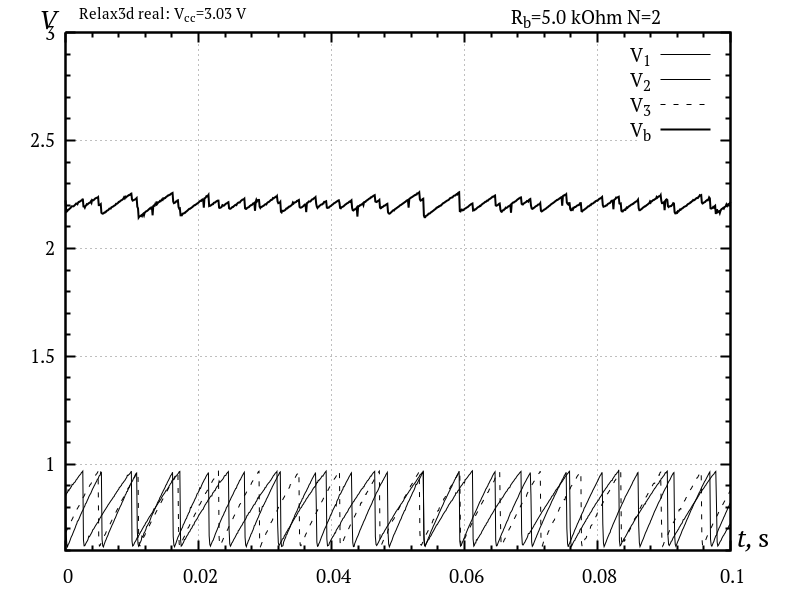
\includegraphics[width=0.6\textwidth]{p/relax3d_t_02.png} }
  \caption{Зависимости $V_b(t)$, $V_i(t)$ для системы рис.~\ref{atu:f:relax3d_schem} при $R_b=\SI{5.0}{\kilo\ohm}$ }
  \label{atu:f:relax3d_t_02}
\end{figure}

В этих условиях спектр $V_b(t)$ практически представляет собой линейную комбинацию спектров
(с соответствующими коэффициентами) отдельных релаксационных
элементов, т.е. набор отдельных частот~(рис.~\ref{atu:f:relax3d_f_02},a).
Аттрактор системы при этом имееет вид достаточно нетипичный для
нехаотрических систем (рис.~\ref{atu:f:relax3d_f_02},b).
Если отношения частот релаксационных элементов
не представляют собой рационально число, что аттрактор
предстваляет собой куб, плотно заполенный по каждой координате в
дипазоне $[ V\Tidx{off} ; V\Tidx{on} ] $.


\begin{figure}[htb!]
  \centerline{
    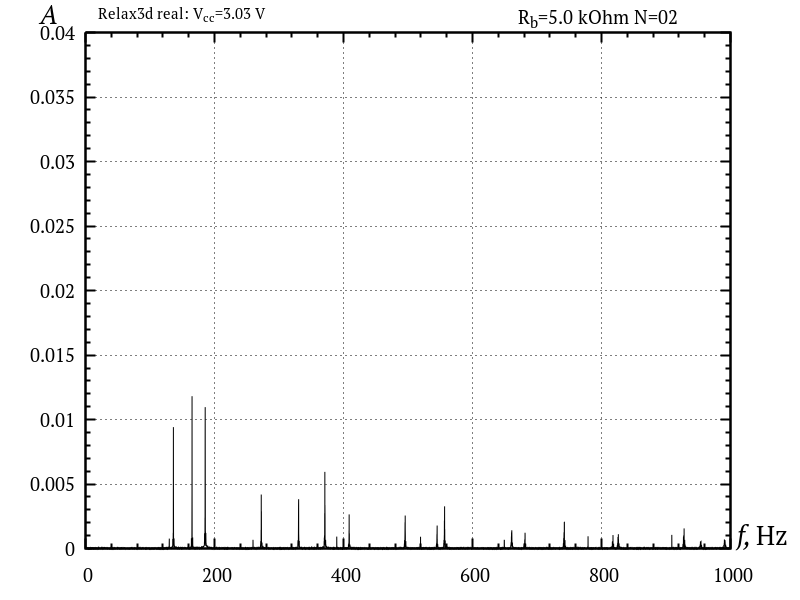
\includegraphics[width=0.48\textwidth]{p/relax3d_f_02.png}
    ~
    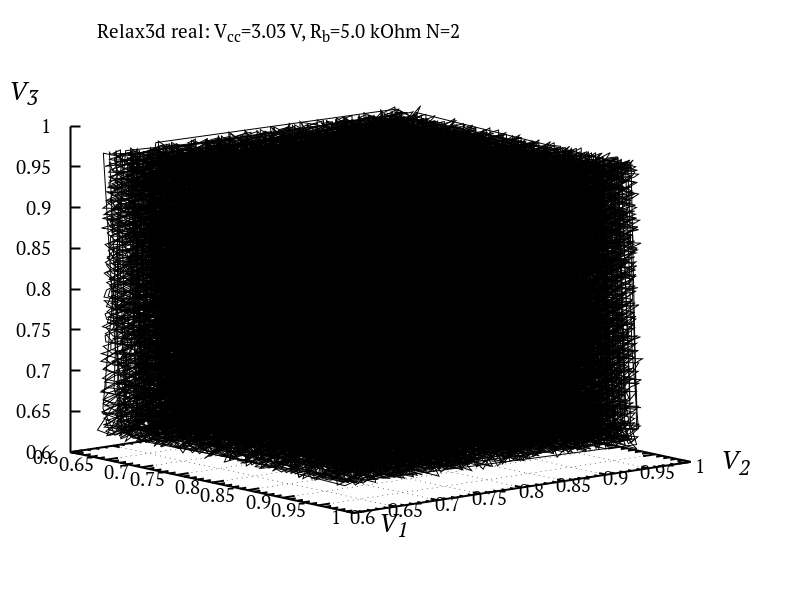
\includegraphics[width=0.48\textwidth]{p/relax3d_v1v2v3_02.png}
  }
  \caption{Спектр $V_b(t)$, и аттрактор для системы рис.~\ref{atu:f:relax3d_schem} при $R_b=\SI{5.0}{\kilo\ohm}$ }
  \label{atu:f:relax3d_f_02}
\end{figure}

При увеличении $R_b$ связь между релаксационными элементами становится более сильной
(рис.~\ref{atu:f:relax3d_t_08}), и при этом возможна ситуация, когда
процесс заряда одного элемента настолько замедляет момент перелючения другого,
что это замедление влиет на все элементы. Возникает состояние ``гонки'',
когда первый подошедший к помонту переключения элемент существенно замедляет второго.
Таким образом, возникает точка бифуркации, когда малые изменения
в исходном состоянии системы приводят к существенным изменением в последующей динамике.
При благоприятных условиях это может приводить к хаотическому поведению.


\begin{figure}[htb!]
  \centerline{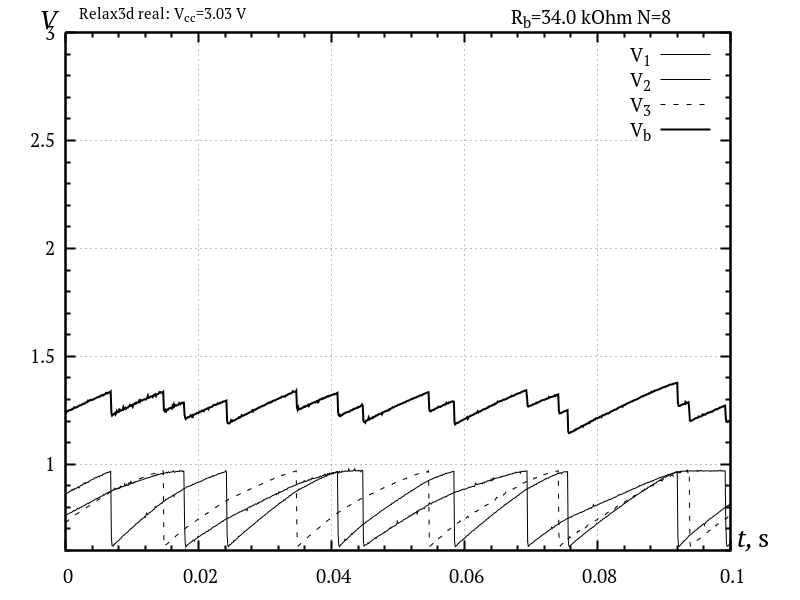
\includegraphics[width=0.6\textwidth]{p/relax3d_t_08.png} }
  \caption{Зависимости $V_b(t)$, $V_i(t)$ для системы рис.~\ref{atu:f:relax3d_schem} при $R_b=\SI{34.0}{\kilo\ohm}$ }
  \label{atu:f:relax3d_t_08}
\end{figure}

При этом спектр системы имеет сплошные участки, подтверждая
хаотичность поведения~(рис.~\ref{atu:f:relax3d_f_08},a).
Аттрактор же системы~(рис.~\ref{atu:f:relax3d_f_08},b),
наоборот, менее плотно заполняет доступное пространство.

\begin{figure}[htb!]
  \centerline{
    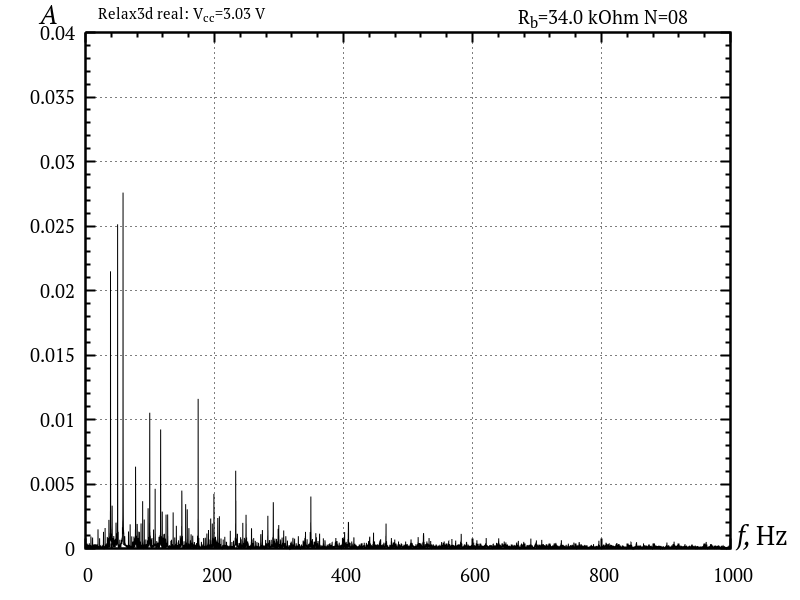
\includegraphics[width=0.48\textwidth]{p/relax3d_f_08.png}
    ~
    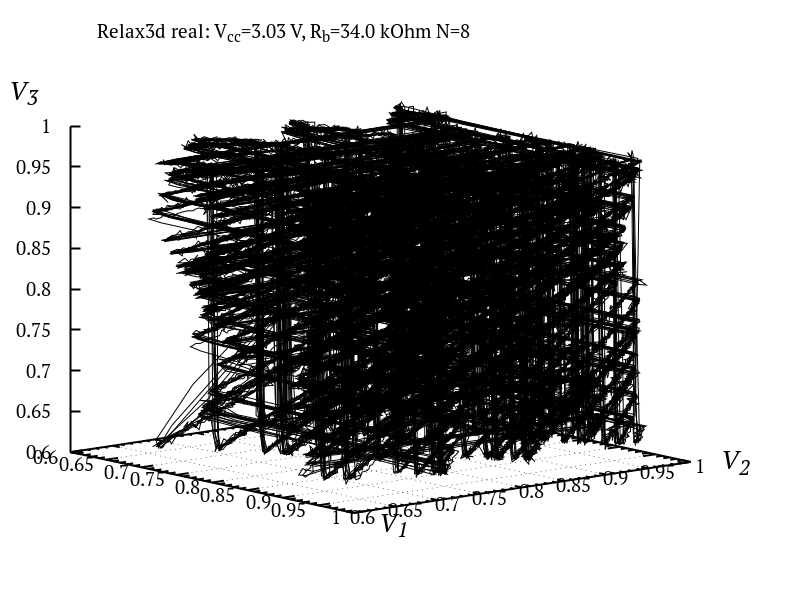
\includegraphics[width=0.48\textwidth]{p/relax3d_v1v2v3_08.png}
  }
  \caption{Спектр $V_b(t)$, и аттрактор для системы рис.~\ref{atu:f:relax3d_schem} при $R_b=\SI{34.0}{\kilo\ohm}$ }
  \label{atu:f:relax3d_f_08}
\end{figure}

Однако, сильная связь между релаксационными элементами
совершенно не обязательно приводит к хаотическому поведению.
При определелённых условиях возможна самосинхронизация
элементов генератора, то есть создаются условия,
эквивалентные рациональному отношению частот отдельных генераторов.
Например, при дальнейшем увеличении $R_b$, снова
возникает сложно-периодическое поведение~(рис.~\ref{atu:f:relax3d_t_09}).

\begin{figure}[htb!]
  \centerline{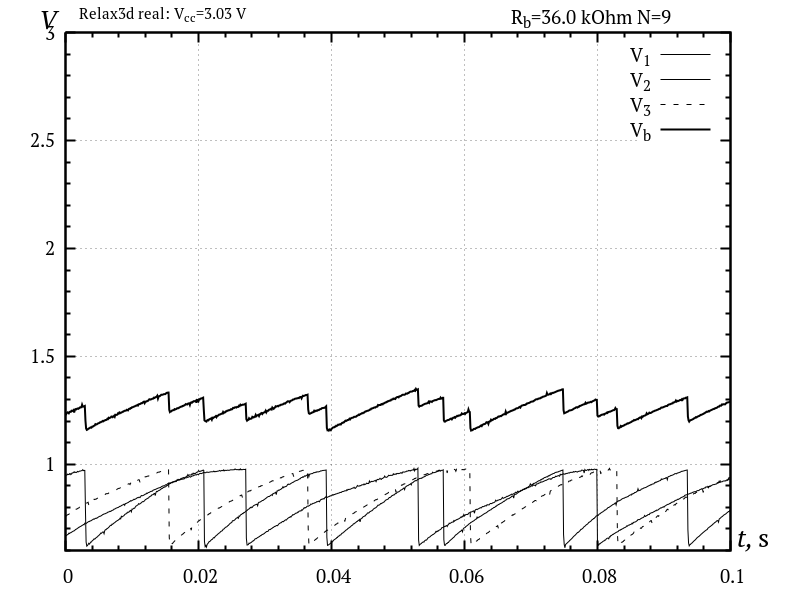
\includegraphics[width=0.6\textwidth]{p/relax3d_t_09.png} }
  \caption{Зависимости $V_b(t)$, $V_i(t)$ для системы рис.~\ref{atu:f:relax3d_schem} при $R_b=\SI{36.0}{\kilo\ohm}$ }
  \label{atu:f:relax3d_t_09}
\end{figure}

Спектр системы становится линейчатым (рис.~\ref{atu:f:relax3d_f_09},a), при этом
часто наблюдается равные расстояния между пиками частот.
Аттрактор становится более вырожденным (рис.~\ref{atu:f:relax3d_f_09},b).

\begin{figure}[htb!]
  \centerline{
    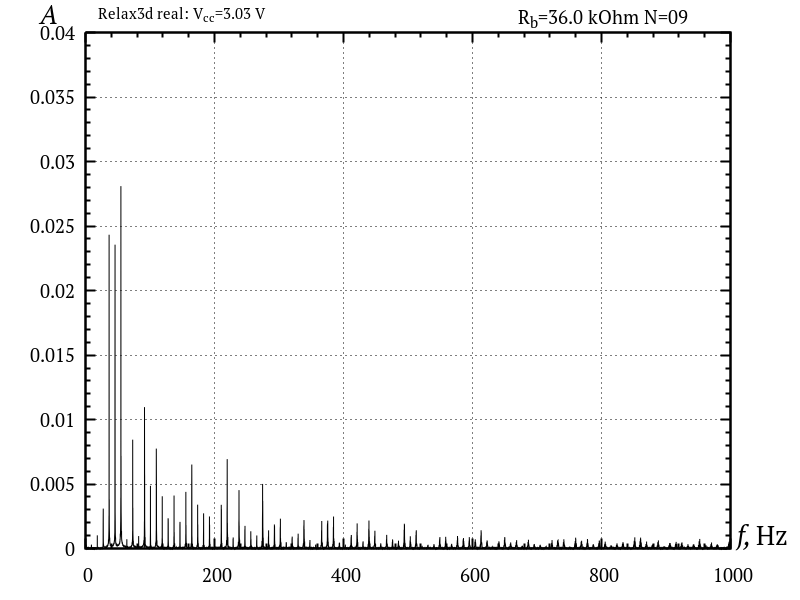
\includegraphics[width=0.48\textwidth]{p/relax3d_f_09.png}
    ~
    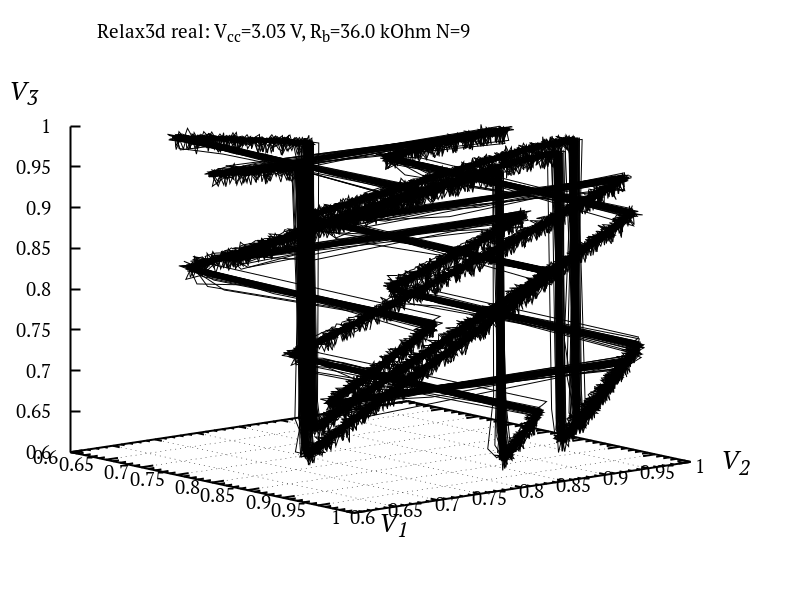
\includegraphics[width=0.48\textwidth]{p/relax3d_v1v2v3_09.png}
  }
  \caption{Спектр $V_b(t)$, и аттрактор для системы рис.~\ref{atu:f:relax3d_schem} при $R_b=\SI{36.0}{\kilo\ohm}$ }
  \label{atu:f:relax3d_f_09}
\end{figure}

С дальнейшим ростом значения параметра $R_b$, сложно-периодический и хаотический
режимы чередуются. В конце концов, возникае режим, когда
один из релаксационных элементов прекращает генерацию~(рис.~\ref{atu:f:relax3d_t_22}).
Этот момент наступает значительно раньше, чем предсказывает
модель. Это связано с тем, что применённый в данной схеме переключающий элемент
при малых токах начинает работать как стабилизатор напряжения.

\begin{figure}[htb!]
  \centerline{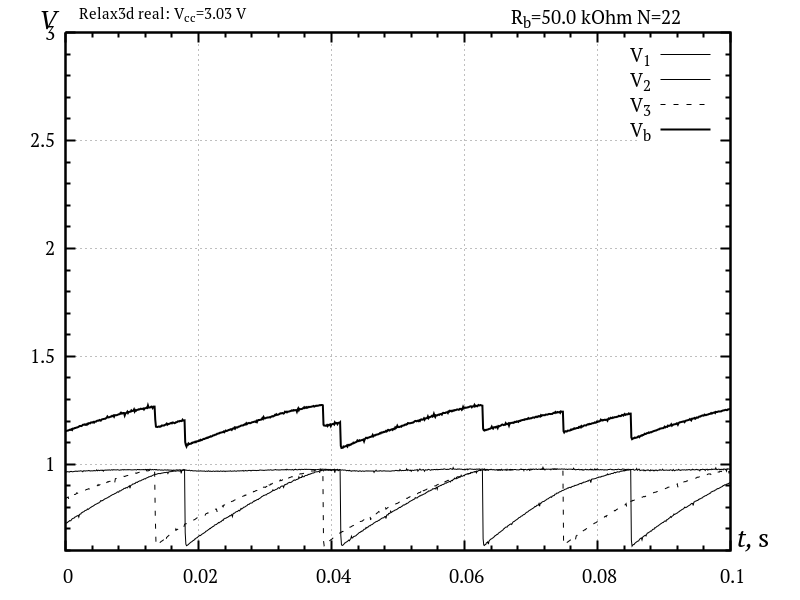
\includegraphics[width=0.6\textwidth]{p/relax3d_t_22.png} }
  \caption{Зависимости $V_b(t)$, $V_i(t)$ для системы рис.~\ref{atu:f:relax3d_schem} при $R_b=\SI{50.0}{\kilo\ohm}$ }
  \label{atu:f:relax3d_t_22}
\end{figure}

Оставшиеся два рабочих релаксационных элемента обеспечивают
достоточно бедный линейчатый спектр~(рис.~\ref{atu:f:relax3d_f_22},a).
Аттратор при этом теряет одно из измерений~(рис.~\ref{atu:f:relax3d_f_22},b),
соответствующее выключившемуся из генерации элементу.

\begin{figure}[htb!]
  \centerline{
    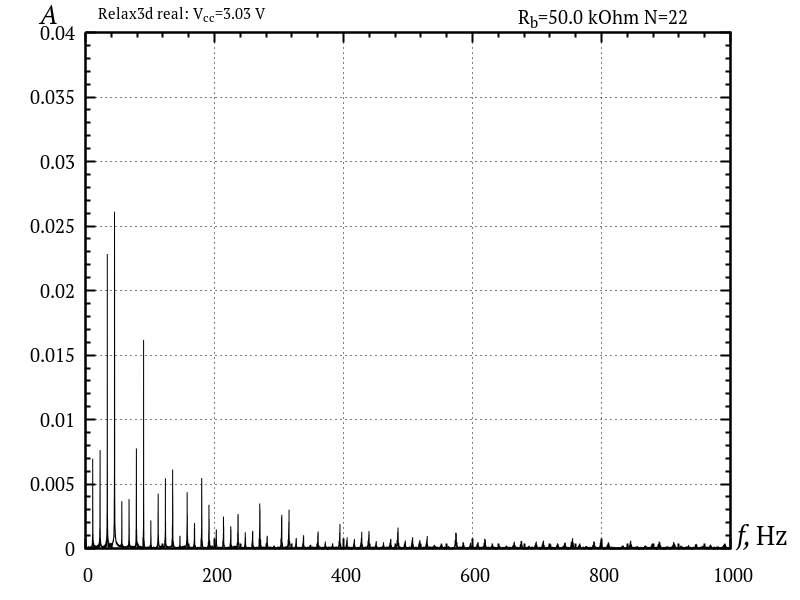
\includegraphics[width=0.48\textwidth]{p/relax3d_f_22.png}
    ~
    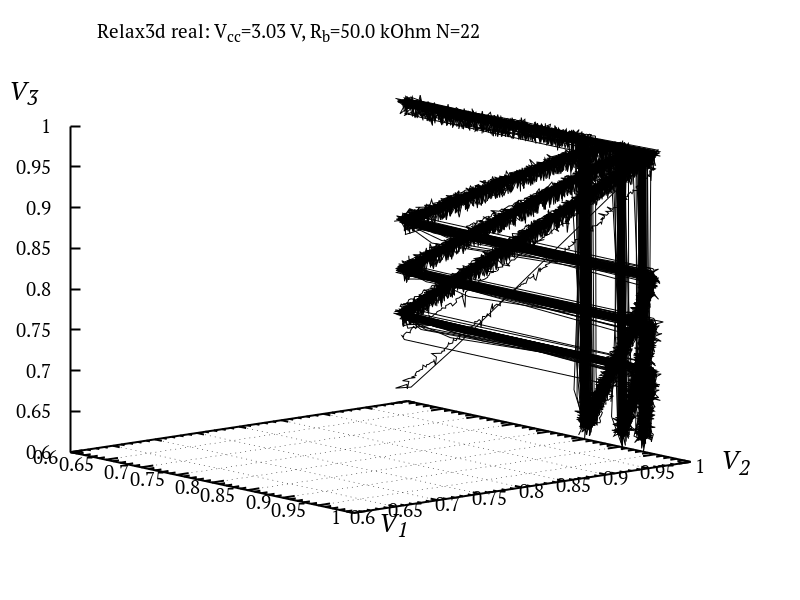
\includegraphics[width=0.48\textwidth]{p/relax3d_v1v2v3_22.png}
  }
  \caption{Спектр $V_b(t)$, и аттрактор для системы рис.~\ref{atu:f:relax3d_schem} при $R_b=\SI{50.0}{\kilo\ohm}$ }
  \label{atu:f:relax3d_f_22}
\end{figure}

Таким образом установлено, что
система электрическая схема которой приведена на рис.~\ref{atu:f:relax3d_schem},
в интервале значений параметра $R_b \in [1;50]\;\SI{}{\kilo\ohm}$
демонстрирует как сложно-периодическое, так и хаотическое поведение,
причём режимы имеют тенденцию к чередованию.

\section{Система из трёх связанных релаксационных генераторов на основе триггеров Шмидта}
\label{atu:sec:relax3ds}

Схемотехническая реализация системы связанных релаксационных генераторов,
рассмотренная в разделе \ref{atu:sec:relax3d}, несмотря на ряд достоинств,
обладает определёнными недостатками. В первую очередь, следует отметить
тот факт, что при относительно высоких значениях величины $R_b$,
как раз при которых связь между отдельными генераторами становится существенной,
релаксационный элемент переключается из колебательного режима в режим
стабилизации напряжения, что не соответствует предназначению данной схемы.
Более того, в этих условиях зависимость тока от напряжения близка к экспоненциальной,
что затрудняет создание адекватной модели. При этом малые изменения параметров,
например, вызванные температурной нестабильностью, приводят к значительным изменением
тока, что также негативно сказывается на адекватности. Ещё один недостаток
заключается в том, что существующими элементами можно изменять напряжение срабатывания
в достаточно узком диапазоне, что затрудняет проведение как экспериментов,
так и моделирования в широком диапазоне параметров. В свою очередь,
это ставит дополнительные вопросы о границах применимости модели, на которые сложно
ответить, опираясь на результаты эксперимента.

Таким образом, возникает задача синтеза схемы системы связанных
релаксационных генераторов, которая бы в минимальной степени была бы
подвержена вышеупомянутым недостаткам.

Одним из достаточно очевидных способов заключается
в разделении переключающего элемента
на измерительную и переключающую части.
В качестве переключающей части можно продолжить использовать биполярный
транзистор. Использование MOSFET транзистора может позволить
значительно уменьшить сопротивление цепи разряда, однако,
учитывая требование к низкому напряжению питания,
обеспечить полное открытие такого транзистора
без применения специальных драйверов достаточно сложно,
а специальные драйверы требуют отдельного питания,
что требует определённых мер предосторожности при подключении АЦП,
и, в свою очередь, могут вносить дополнительные искажения.

В качестве измерительного элемента можно использовать
подходящую по условиям бистабильную схему,
чувствительную к напряжению, например триггер Шмидта.
Если существует необходимость управлять
значениями величин
$V\Tidx{on}$, $V\Tidx{off}$,
то триггер следует реализовывать,
используя операционные усилители~[Хоровиц].
При фиксированных значения этих параметров,
можно использовать триггеры Шмидта в интегральном исполнении,
подобрав соответствующую серию.
У учётом вышеупомянутых требований,
были выбраны микросхемы серии 74HC14N,
представляющие собой 6 элементов ``НЕ''
с триггером Шмидта на входе. Комбинируя их по два,
получим три требуемые измерительные элемента.
Получившаяся схема представлена на рис.~\ref{atu:f:relax3ds_schem}.


\begin{figure}[htb!]
  \centerline{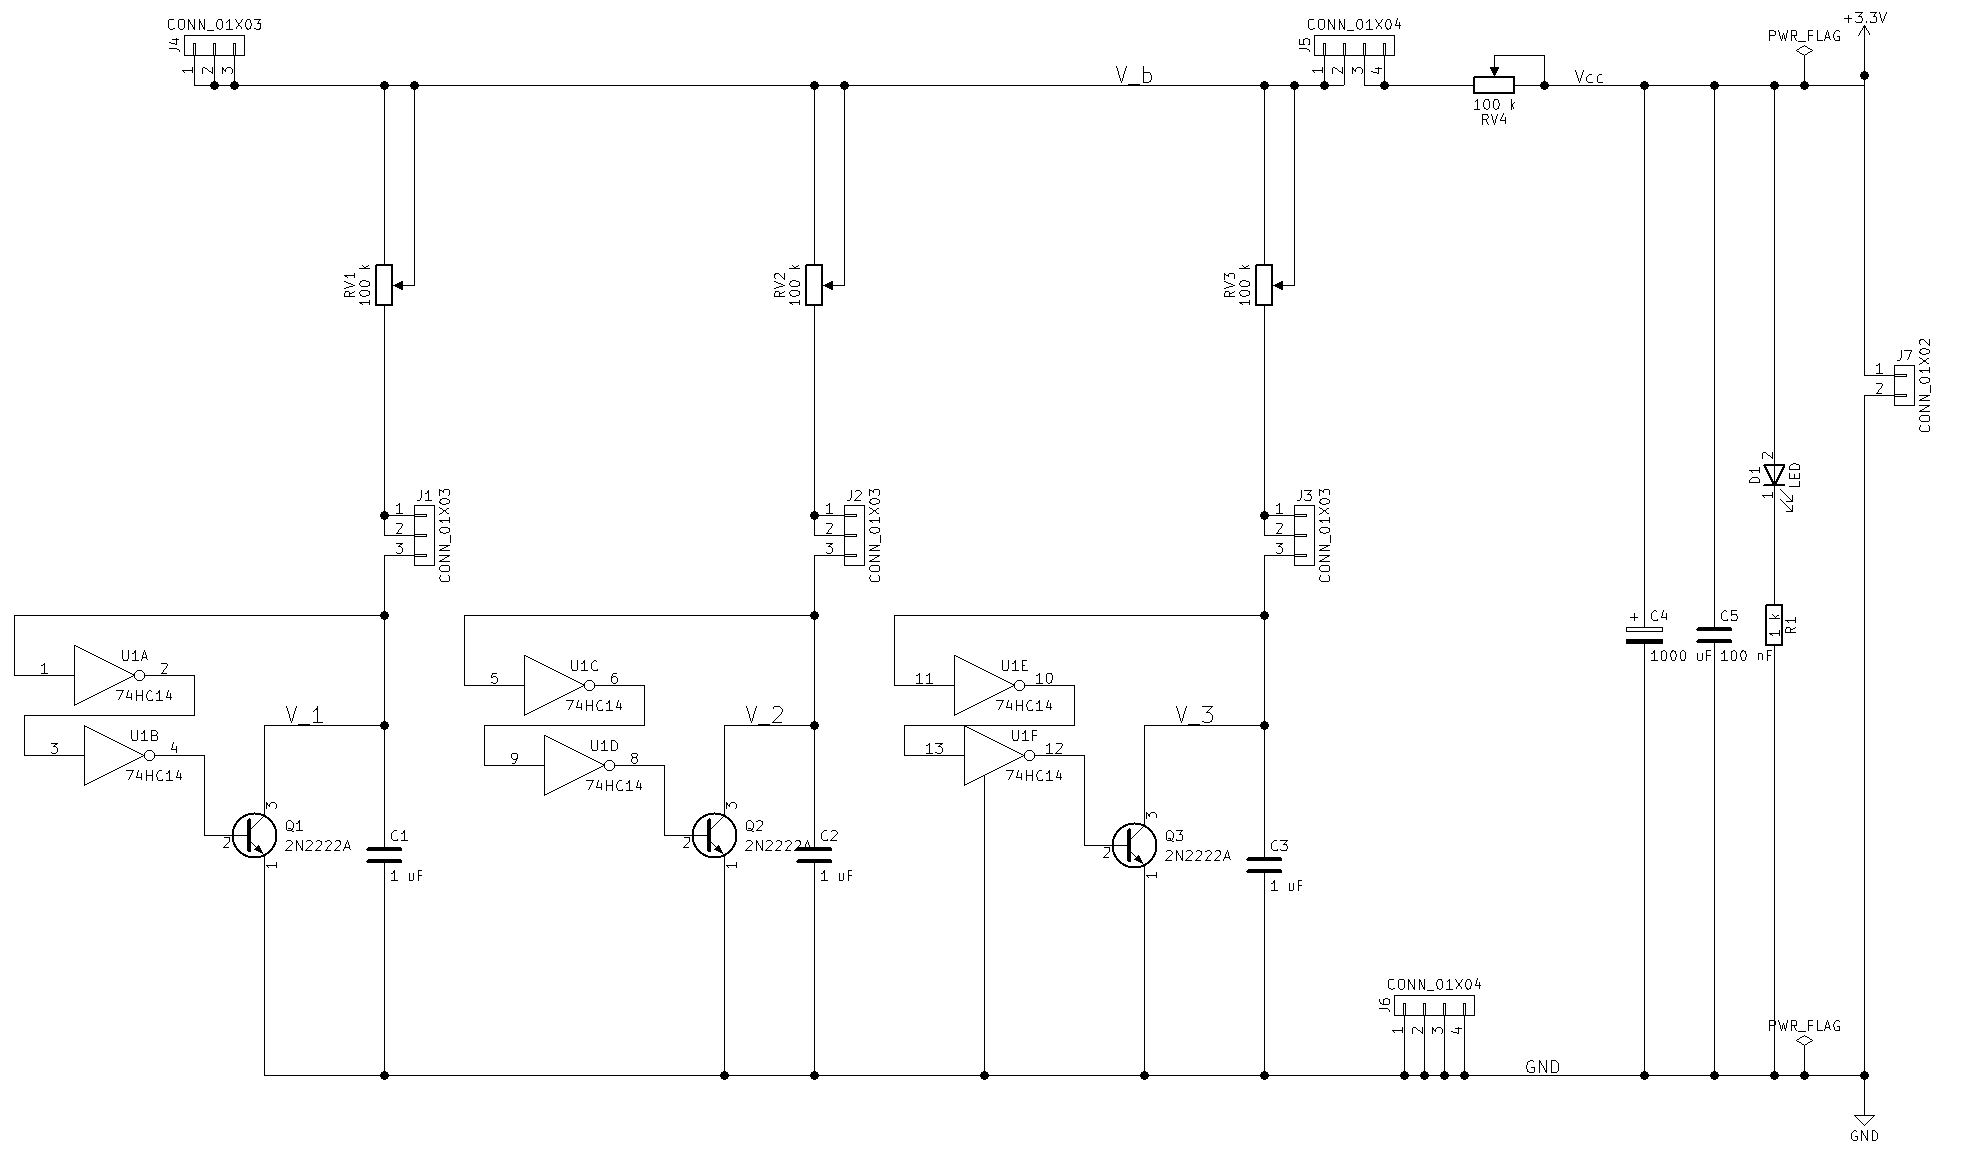
\includegraphics[width=0.9\textwidth]{p/relax3ds_schem.png} }
  \caption{Электрическая схема \RelaxShIi}
  \label{atu:f:relax3ds_schem}
\end{figure}

Принципиальна эта схема не отличается от изображённой на рис.(рис.~\ref{atu:f:relax3d_schem}).
Все вспомогательные элементы исполняют аналогичную роль.
При этом существуют и определённые отличия.
Напряжения срабатывания переключающего элемента
у данной схемы отличаются, и определяются
параметрами триггера.
Согласно документации, для указанной микросхемы
при $V\Tidx{cc} = \SI{3}{\volt} $
допустимые диапазоны определяются так:
$V\Tidx{off} \in [ 0.51; 1.35 ] \SI{}{\volt}$,
$V\Tidx{on}  \in [ 1.08; 2.16 ] \SI{}{\volt}$.
Диапазоны существенно отличаются от таковых для предыдущей схемы.
Более того, разброс допустимых параметров очень широк,
и, теоретически, возможно ситуация, когда некоторые из релаксационных
элементов не будут работать.
Тем не менее, при реальных измерениях
для одного конкретного экземпляра
разброс оказался не так велик:
$V\Tidx{off,1} = \SI{1.10}{\volt}$,
$V\Tidx{off,2} = \SI{1.05}{\volt}$,
$V\Tidx{off,3} = \SI{1.02}{\volt}$,
$V\Tidx{on,1}  = \SI{1.87}{\volt}$,
$V\Tidx{on,2}  = \SI{1.83}{\volt}$,
$V\Tidx{on,3}  = \SI{1.81}{\volt}$.
Различия, несмотря на то, что они заметно меньше, чем допустимы по официальной документации,
тем не менее существенно больше, чем в предыдущей схеме, что требует
обязательного учёта в модели.

Аналогично предыдущей схеме, рассмотрим её динамику при
изменении $R_b$, выделяя аналогичные режимы.


При малых
значениях $R_b$
совершенно аналогично наблюдаются практически независимые
колебания~(рис.~\ref{atu:f:relax3ds_t_05151}).
Однако, из-за повышения напряжений переключения,
колебания величины $V\Tidx{b}$
выражены сильнее.

\begin{figure}[htb!]
  \centerline{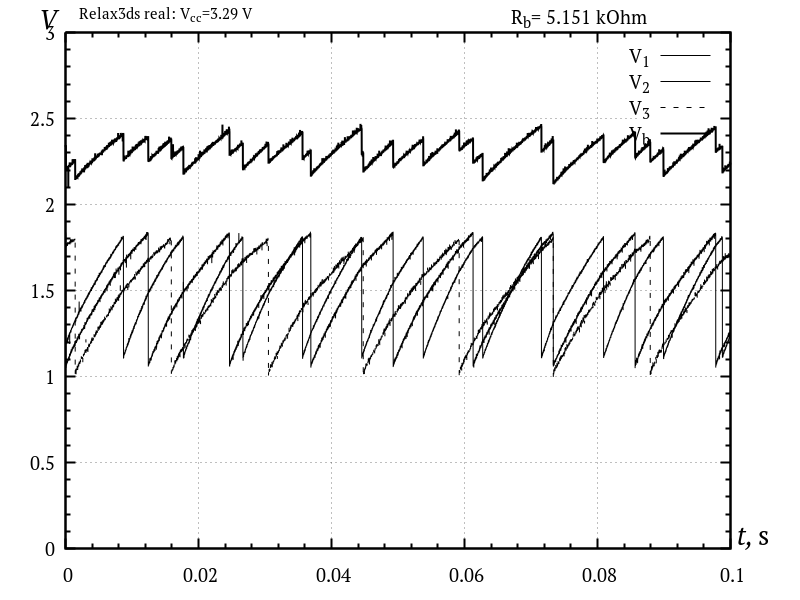
\includegraphics[width=0.6\textwidth]{p/relax3ds_t_005151.png} }
  \caption{Зависимости $V_b(t)$, $V_i(t)$ для системы рис.~\ref{atu:f:relax3ds_schem} при $R_b=\SI{5.15}{\kilo\ohm}$ }
  \label{atu:f:relax3ds_t_05151}
\end{figure}


Из-за более сильной связи между элементами,
наблюдается уширение спектральных линий~(рис.~\ref{atu:f:relax3ds_f_05151}).
Аттрактор предстваляет собой прямоугольный параллелепипед, достаточно плотно заполненный по каждой координате в
дипазоне $[ V\Tidx{off,i} ; V\Tidx{on,i} ] $.


\begin{figure}[htb!]
  \centerline{
    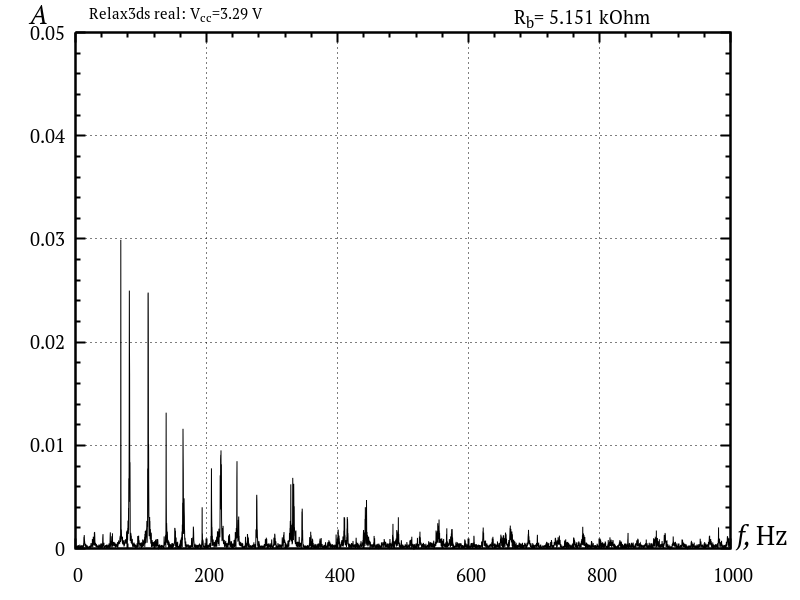
\includegraphics[width=0.48\textwidth]{p/relax3ds_f_005151.png}
    ~
    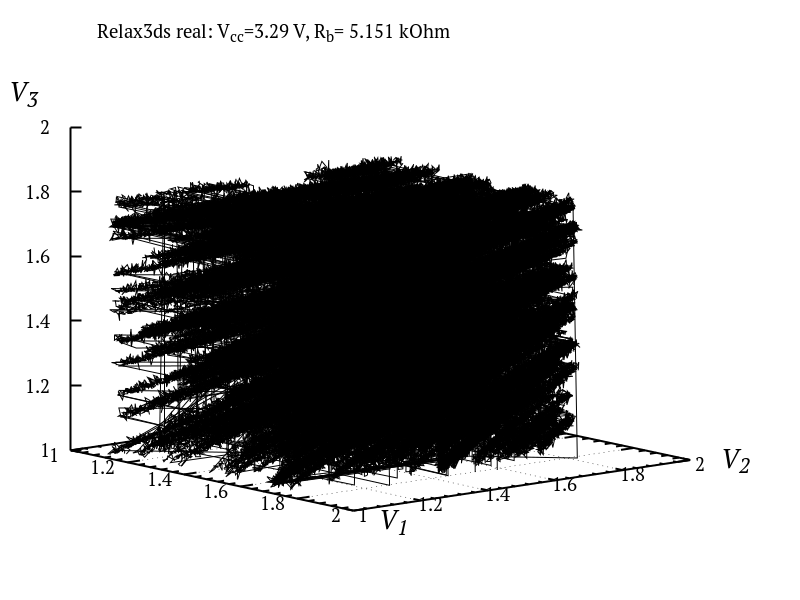
\includegraphics[width=0.48\textwidth]{p/relax3ds_v1v2v3_005151.png}
  }
  \caption{Спектр $V_b(t)$, и аттрактор для системы рис.~\ref{atu:f:relax3ds_schem} при $R_b=\SI{5.15}{\kilo\ohm}$ }
  \label{atu:f:relax3ds_f_05151}
\end{figure}

Усиление связи приводит к выраженному хаотическому поведению
(рис.~\ref{atu:f:relax3ds_t_13246}).

\begin{figure}[htb!]
  \centerline{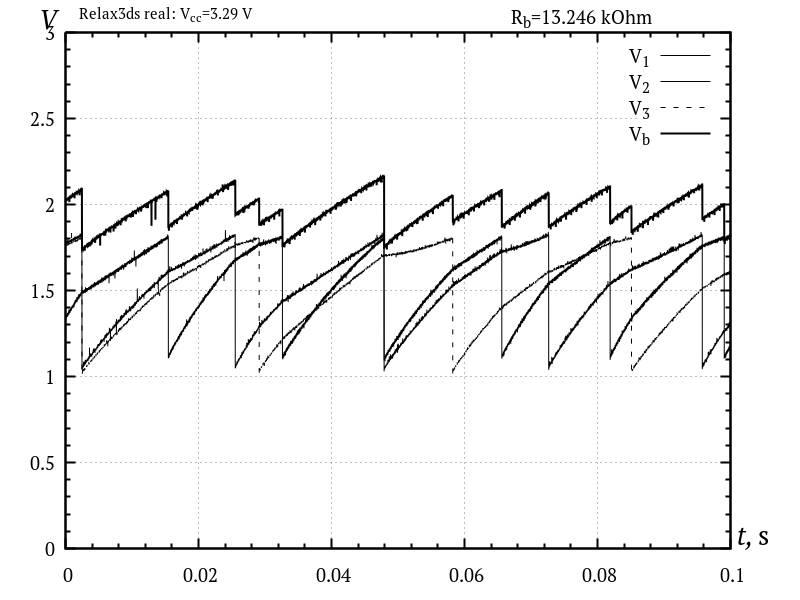
\includegraphics[width=0.6\textwidth]{p/relax3ds_t_013246.png} }
  \caption{Зависимости $V_b(t)$, $V_i(t)$ для системы рис.~\ref{atu:f:relax3ds_schem} при $R_b=\SI{13.25}{\kilo\ohm}$ }
  \label{atu:f:relax3ds_t_13246}
\end{figure}

Сплошные участки спектра~(рис.~\ref{atu:f:relax3ds_f_13246},a)
являются хорошим индикатором.
Аттрактор выглядит аналогично~(рис.~\ref{atu:f:relax3ds_f_13246},b).

\begin{figure}[htb!]
  \centerline{
    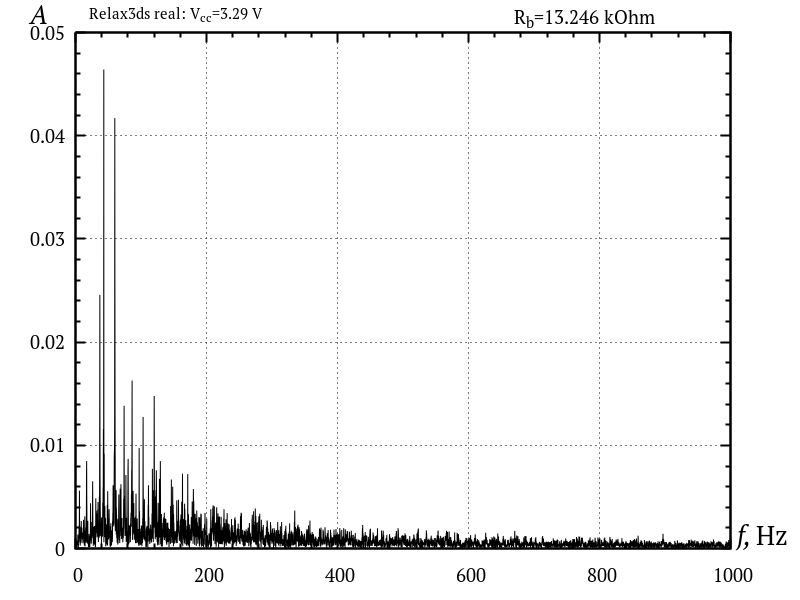
\includegraphics[width=0.48\textwidth]{p/relax3ds_f_013246.png}
    ~
    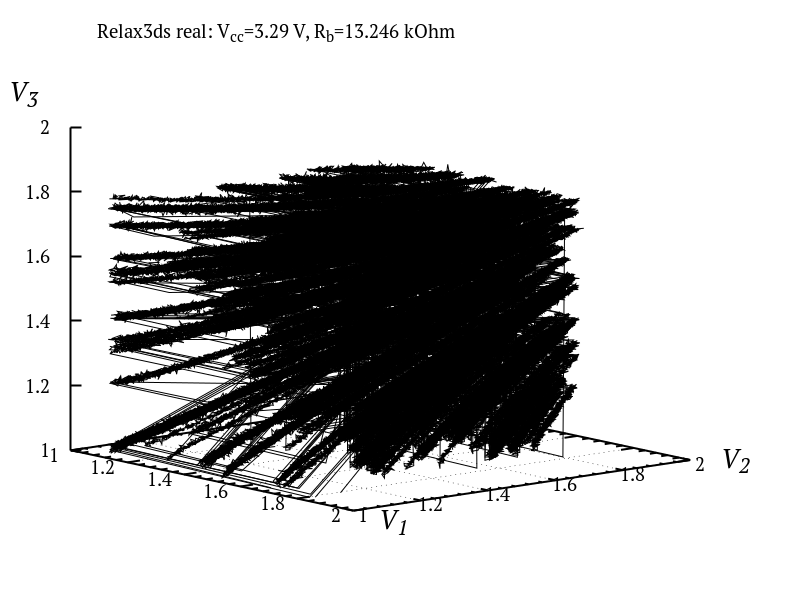
\includegraphics[width=0.48\textwidth]{p/relax3ds_v1v2v3_013246.png}
  }
  \caption{Спектр $V_b(t)$, и аттрактор для системы рис.~\ref{atu:f:relax3ds_schem} при $R_b=\SI{13.25}{\kilo\ohm}$ }
  \label{atu:f:relax3ds_f_13246}
\end{figure}


Определённые значения $R_b$ переводят систему в сложно-периодический режим
(рис.~\ref{atu:f:relax3ds_t_14718}).

\begin{figure}[htb!]
  \centerline{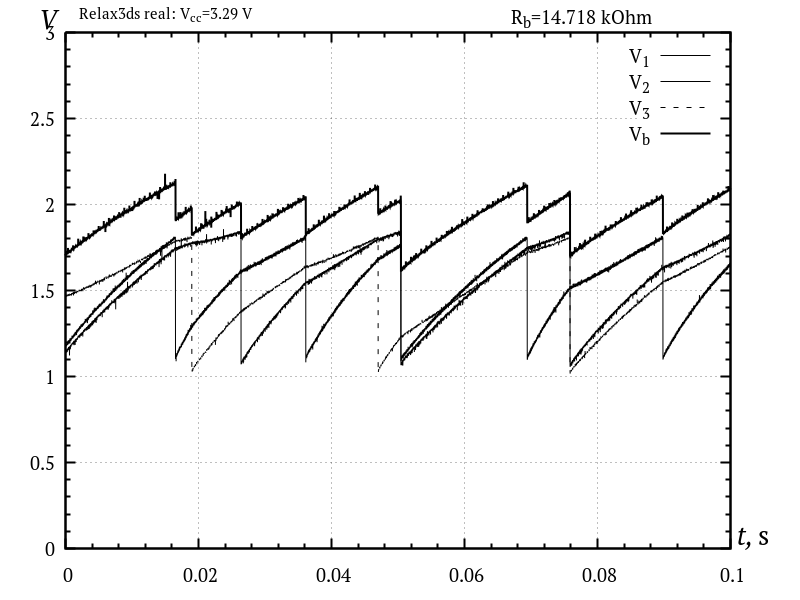
\includegraphics[width=0.6\textwidth]{p/relax3ds_t_014718.png} }
  \caption{Зависимости $V_b(t)$, $V_i(t)$ для системы рис.~\ref{atu:f:relax3ds_schem} при $R_b=\SI{14.72}{\kilo\ohm}$ }
  \label{atu:f:relax3ds_t_14718}
\end{figure}

Спектр~(рис.~\ref{atu:f:relax3ds_f_14718},a)
подтверждает отсутствие хаоса,
несмотря еа тонкую линейчатую структуру.
Аттрактор принципиально не изменяется~(рис.~\ref{atu:f:relax3ds_f_14718},b),
но имеет менее плотное заполнение.

\begin{figure}[htb!]
  \centerline{
    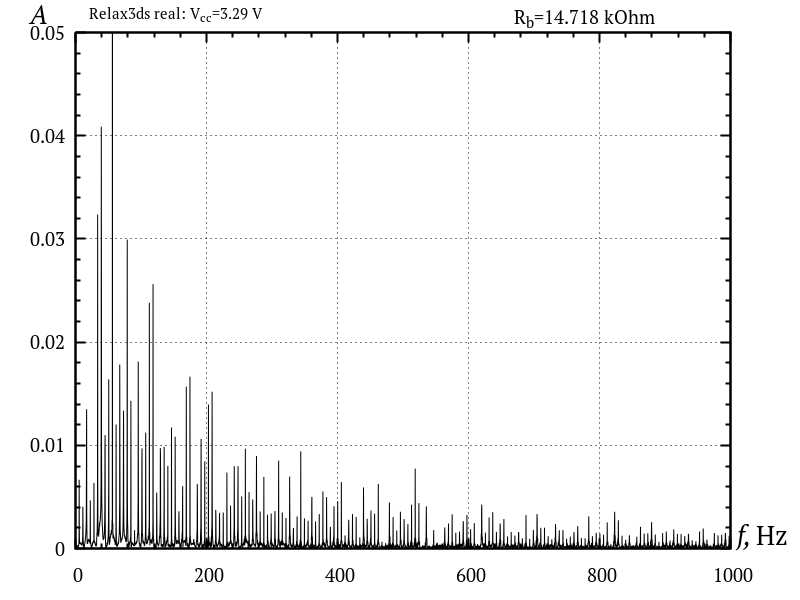
\includegraphics[width=0.48\textwidth]{p/relax3ds_f_014718.png}
    ~
    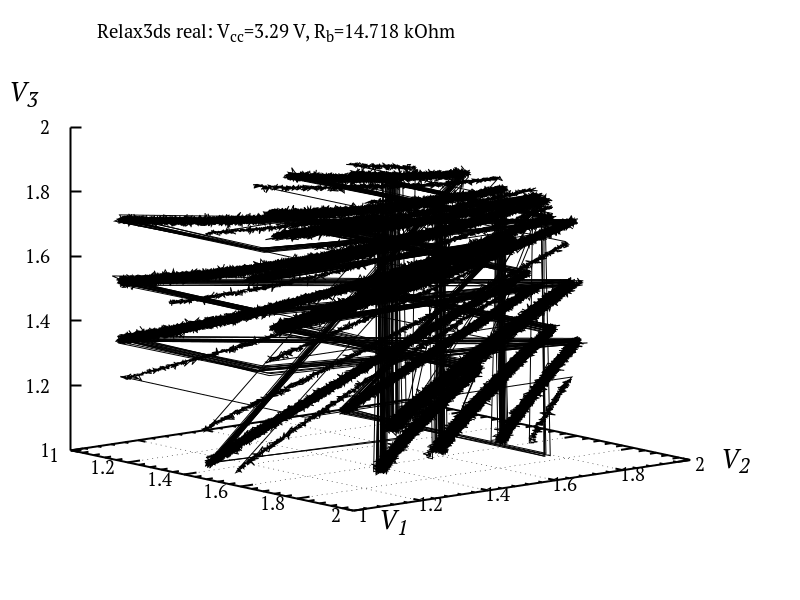
\includegraphics[width=0.48\textwidth]{p/relax3ds_v1v2v3_014718.png}
  }
  \caption{Спектр $V_b(t)$, и аттрактор для системы рис.~\ref{atu:f:relax3ds_schem} при $R_b=\SI{14.72}{\kilo\ohm}$ }
  \label{atu:f:relax3ds_f_14718}
\end{figure}

Высокие значения $R_b$, в отличие от предыдуще системы,
не приводят в быстрому выключению одного из релаксационных
эелементов, при этом может наблюдаться как мложно-периодическе,
так и хаотическое поведение
(рис.~\ref{atu:f:relax3ds_t_36060}).

\begin{figure}[htb!]
  \centerline{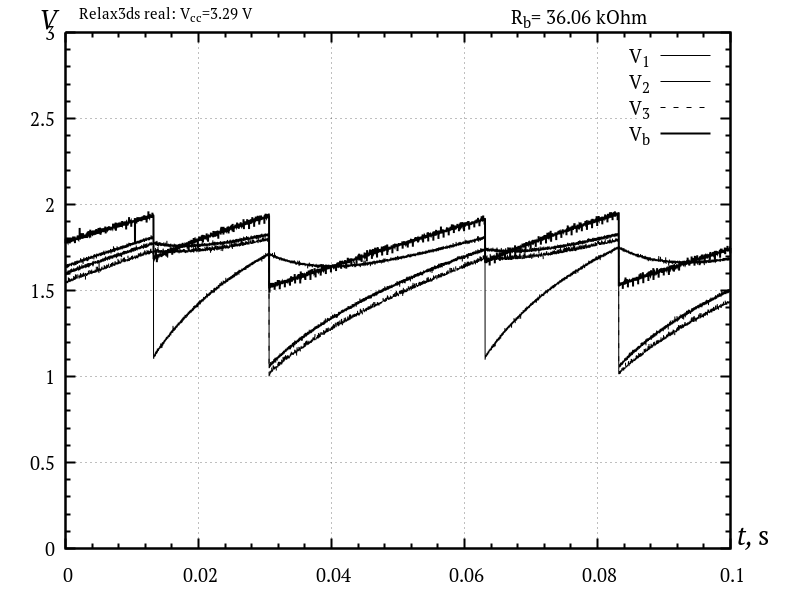
\includegraphics[width=0.6\textwidth]{p/relax3ds_t_036060.png} }
  \caption{Зависимости $V_b(t)$, $V_i(t)$ для системы рис.~\ref{atu:f:relax3ds_schem} при $R_b=\SI{36.06}{\kilo\ohm}$ }
  \label{atu:f:relax3ds_t_36060}
\end{figure}

Спектры могут быть как сплошными~(рис.~\ref{atu:f:relax3ds_f_36060},a)
так и линейчатые.
Аттракторы имеют более простую структуру~(рис.~\ref{atu:f:relax3ds_f_36060},b),
при этом реализуя как и простые эквиваленты фигур Лиссажу,
так и фигуры с плотным заполнением.

\begin{figure}[htb!]
  \centerline{
    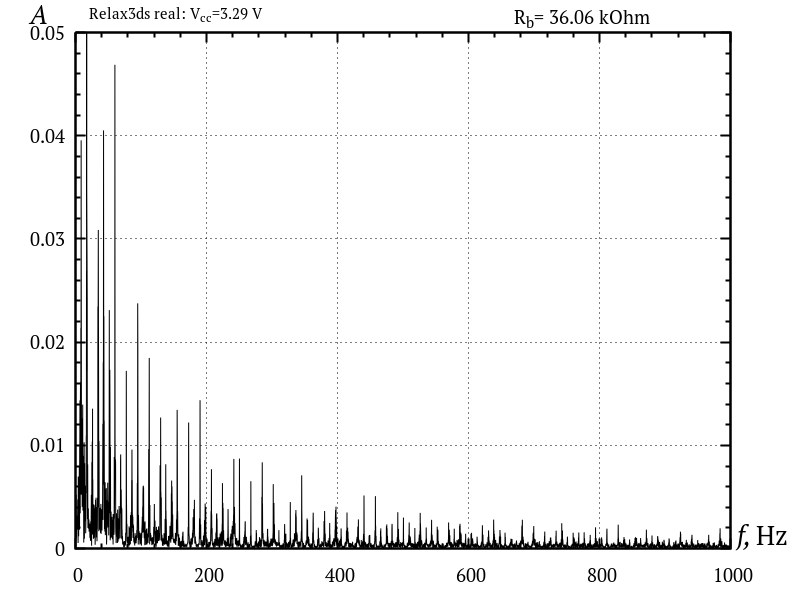
\includegraphics[width=0.48\textwidth]{p/relax3ds_f_036060.png}
    ~
    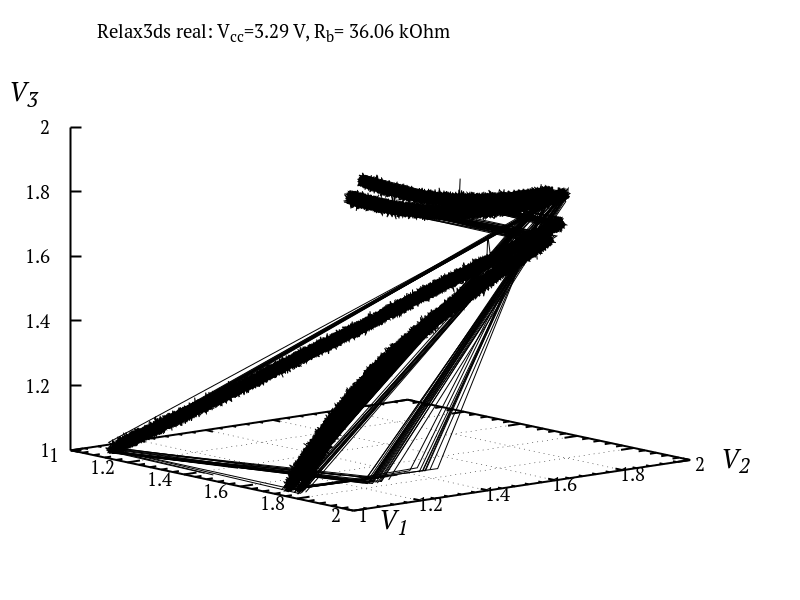
\includegraphics[width=0.48\textwidth]{p/relax3ds_v1v2v3_036060.png}
  }
  \caption{Спектр $V_b(t)$, и аттрактор для системы рис.~\ref{atu:f:relax3ds_schem} при $R_b=\SI{36.06}{\kilo\ohm}$ }
  \label{atu:f:relax3ds_f_36060}
\end{figure}

В целом обе схемы, несмотря на различия, имеют сходные приципы поведения
в достаточно широком дипазоне значений параметра $R_b$.
Существенная разница проявляется при высоких значениях $R_b$,
при этом, очевидно, требуется или уточнение модели, или же
не использование данных режимов, которые в этом контексте не представляют
особого интереса.



\section{Модели систем из трёх связанных релаксационных генераторов}

\begin{equation}
  \begin{cases}
    V_b = V_{cc} - R_b ( I_1 + I_2 + I_3 ), \\
      C_1 \dot{V}_1 = \frac{V_b-V_1}{R_{v1}} - \frac{V_1}{R_1} \mathrm{On}_1() - I_{1,\mathrm{leak}}(V_1), \\
      C_2 \dot{V}_2 = \frac{V_b-V_2}{R_{v2}} - \frac{V_2}{R_2} \mathrm{On}_2() - I_{2,\mathrm{leak}}(V_2), \\
      C_3 \dot{V}_3 = \frac{V_b-V_3}{R_{v3}} - \frac{V_3}{R_3} \mathrm{On}_3() - I_{3,\mathrm{leak}}(V_3), \\
      I_i = \frac{V_b-V_i}{R_{vi}}.
  \end{cases}.
    \label{atu:eq:relax3}
\end{equation}

Параметры: \\
$R_b$ --- сопротивление в цепи питания (идентифицируемый параметр), \\
$C_i$ --- ёмкости кождого из релаксационных генераторов, \\
$R_{vi}$ --- сопротивления зарядки релаксационных генераторов, \\
$R_{i}$ --- сопротивления зарядки релаксационных генераторов, \\
$I_{i,\mathrm{leak}}$ --- токи утечки.

Функции $ \mathrm{On}_i() $ определяют моменты переключения генераторов,
задаются алгоритмически (гистерезис). Определяются параметрами
$V_{on}$, $V_{off}$.

\begin{equation}
  \begin{cases}
    V_b = V_{cc} - R_b ( I_1 + I_2 + I_3 ), \\
      C_1 \dot{V}_1 = \frac{V_b-V_1}{R_{v1}} - \frac{V_1}{R_1} \mathrm{On}_1() - \frac{V_1}{R_1+R_{1,\mathrm{leak}}}, \\
      C_2 \dot{V}_2 = \frac{V_b-V_2}{R_{v2}} - \frac{V_2}{R_2} \mathrm{On}_2() - \frac{V_2}{R_2+R_{2,\mathrm{leak}}}, \\
      C_3 \dot{V}_3 = \frac{V_b-V_3}{R_{v3}} - \frac{V_3}{R_3} \mathrm{On}_3() - \frac{V_3}{R_3+R_{3,\mathrm{leak}}}, \\
      I_i = \frac{V_b-V_i}{R_{vi}}.
  \end{cases}.
    \label{atu:eq:relax3_linleak}
\end{equation}

$R_{i,\mathrm{leak}}$ --- сопротивления утечки.



\section{Критерии идентификации систем из трёх связанных релаксационных генераторов}

\begin{figure}[htb!]
  \centerline{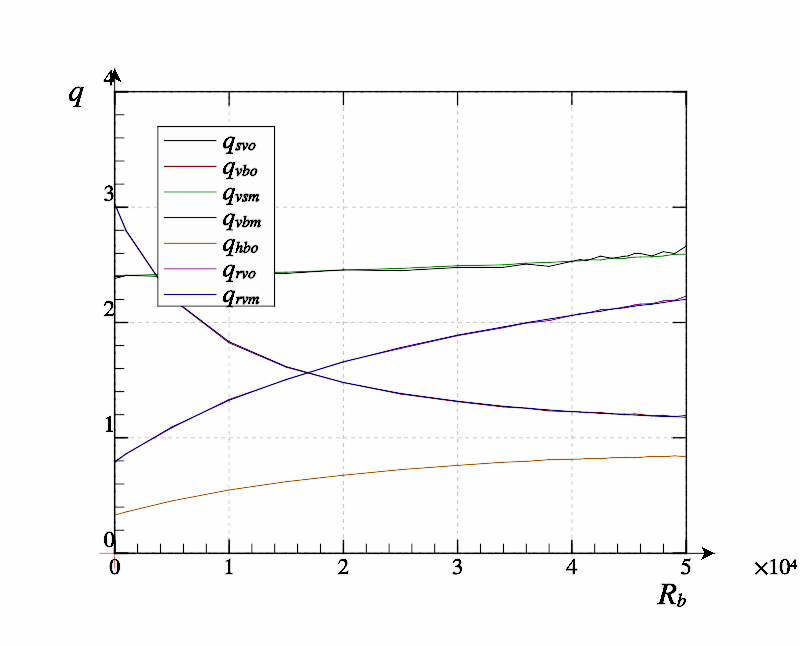
\includegraphics[width=0.7\textwidth]{p/relax3_read_q-p_q1.png} }
  \caption{Зависимости для рассмативаетмых критериев идентификации для системы релаксационных генераторов на паре комплиментарных транзисторов}
  \label{atu:f:relax3d_q}
\end{figure}

\begin{figure}[htb!]
  \centerline{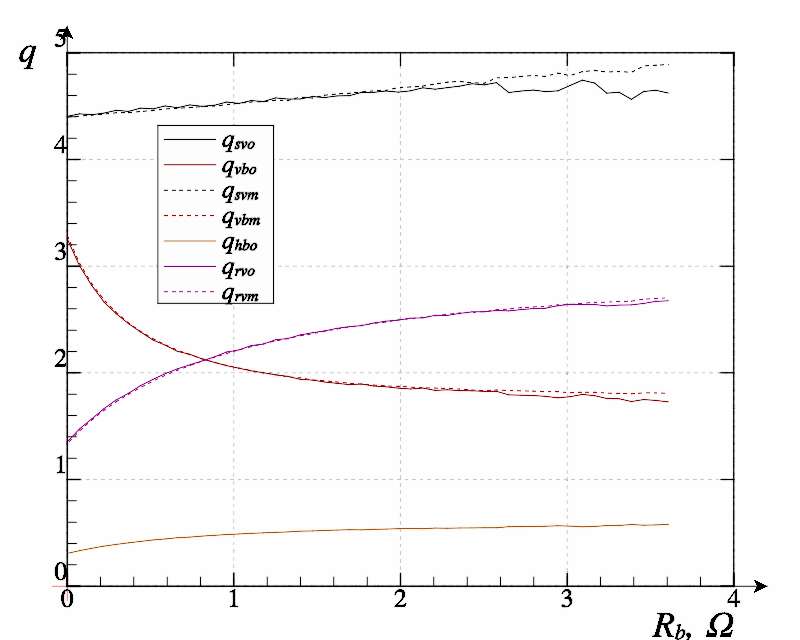
\includegraphics[width=0.7\textwidth]{p/relax3ds_read_q-p_q1.png} }
  \caption{Зависимости для рассмативаетмых критериев идентификации для системы релаксационных генераторов на триггерах Шмидта}
  \label{atu:f:relax3ds_q}
\end{figure}

\section{Идентификация параметра системы из трёх связанных релаксационных генераторов}

\begin{figure}[htb!]
  \centerline{
    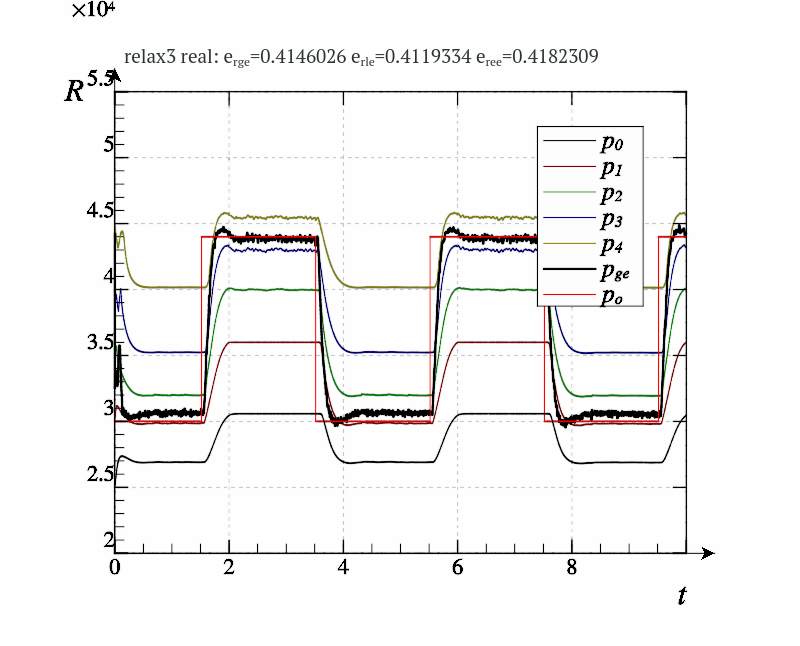
\includegraphics[width=0.45\textwidth]{p/relax3_read_id2-p_p_03.png}
    \hfill
    \includegraphics[width=0.45\textwidth]{p/relax3_read_id2-p_pp_03.png}
  }
  \caption{Идентификация }
  \label{atu:f:relax3d_id}
\end{figure}

\begin{figure}[htb!]
  \centerline{
    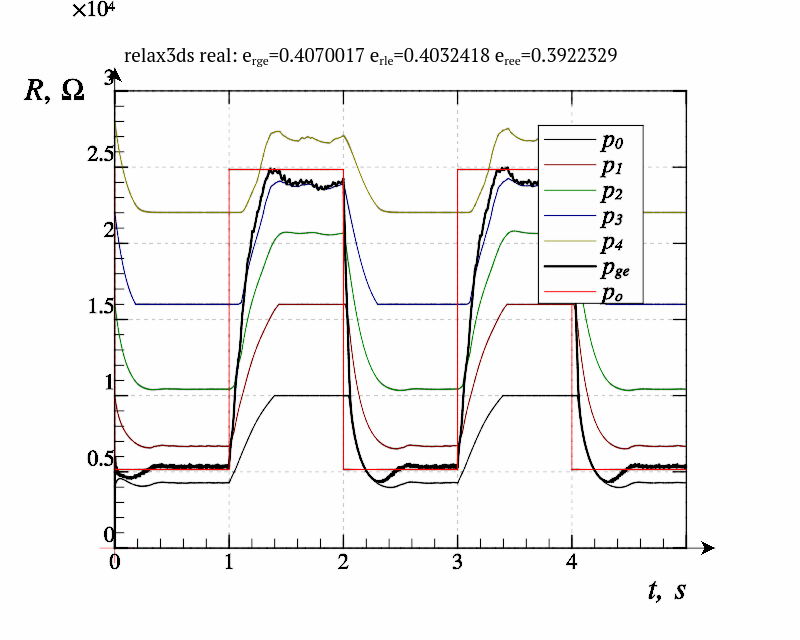
\includegraphics[width=0.45\textwidth]{p/relax3d_read_id2_0-p_p.png}
    \hfill
    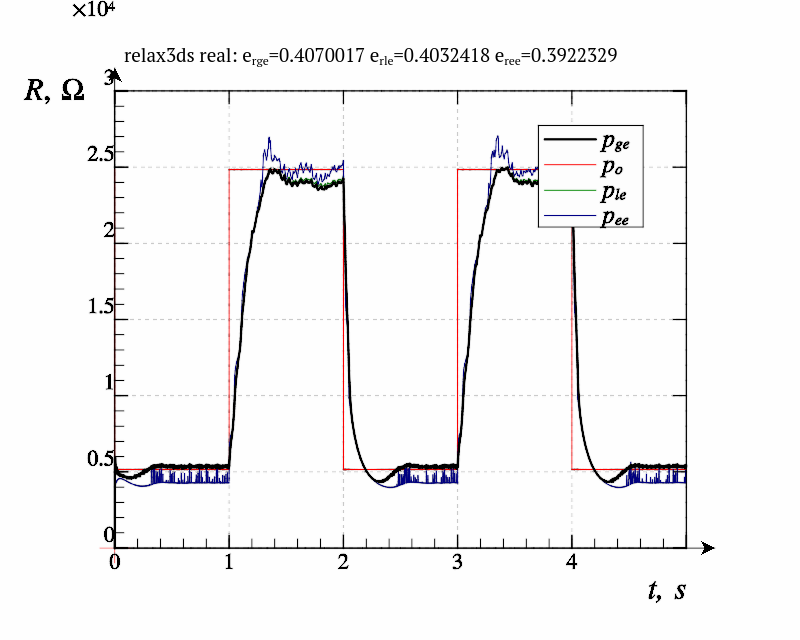
\includegraphics[width=0.45\textwidth]{p/relax3d_read_id2_0-p_pp.png}
  }
  \caption{Идентификация 3ds 0}
  \label{atu:f:relax3ds_id_0}
\end{figure}

\begin{figure}[htb!]
  \centerline{
    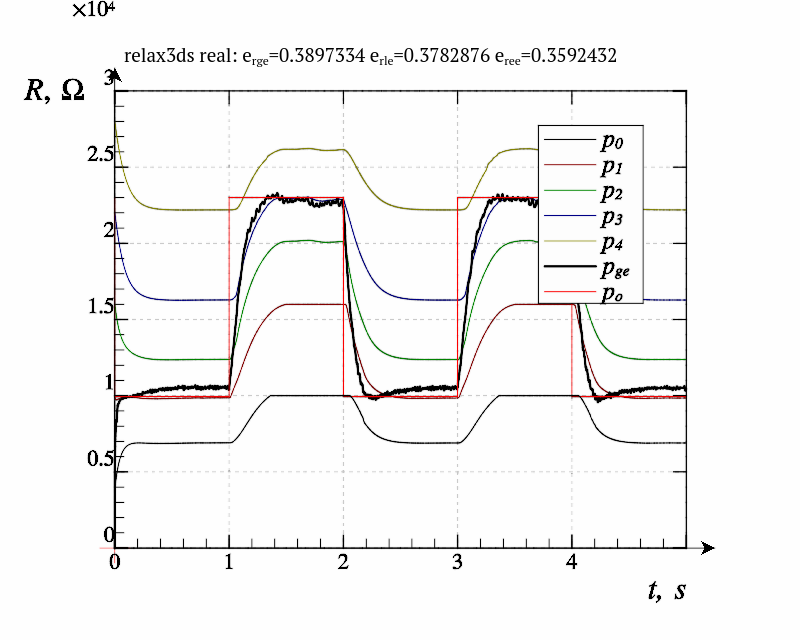
\includegraphics[width=0.45\textwidth]{p/relax3d_read_id2_1-p_p.png}
    \hfill
    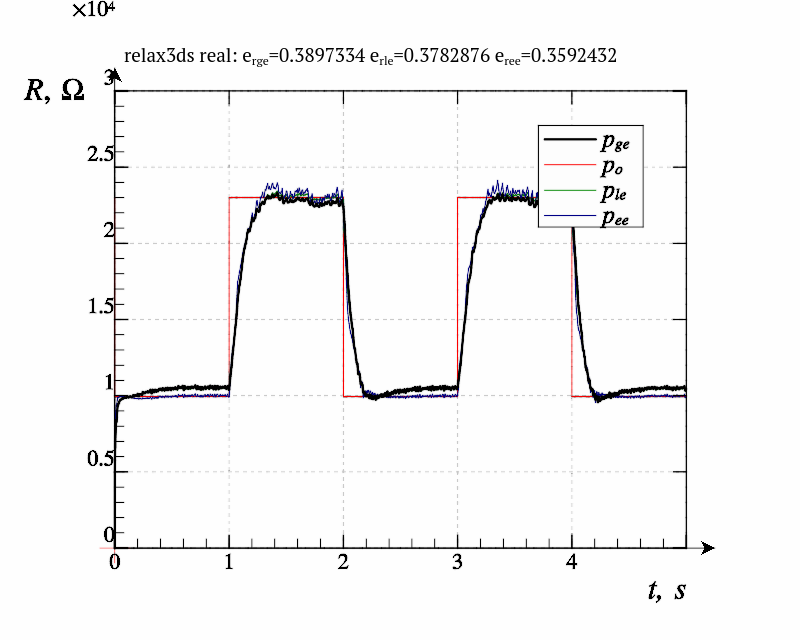
\includegraphics[width=0.45\textwidth]{p/relax3d_read_id2_1-p_pp.png}
  }
  \caption{Идентификация 3ds 1}
  \label{atu:f:relax3ds_id_1}
\end{figure}

\begin{figure}[htb!]
  \centerline{
    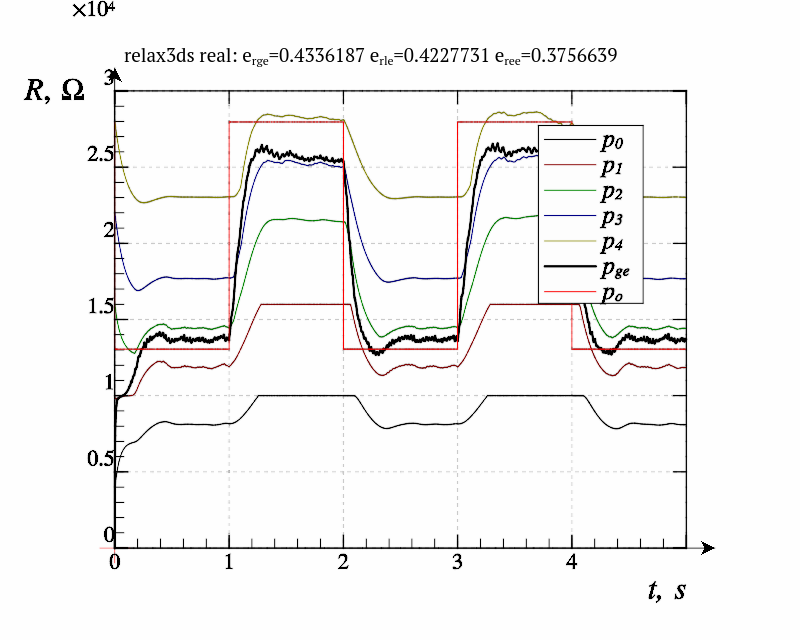
\includegraphics[width=0.45\textwidth]{p/relax3d_read_id2_2-p_p.png}
    \hfill
    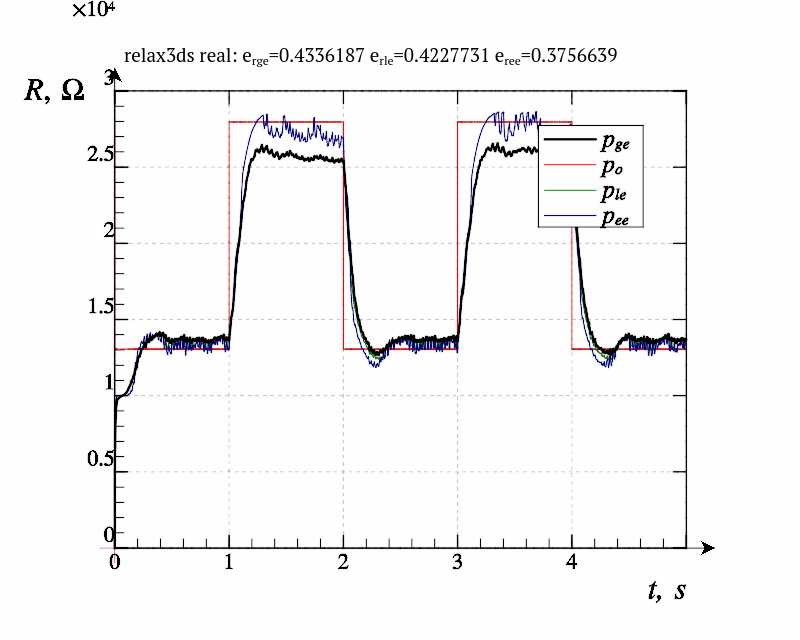
\includegraphics[width=0.45\textwidth]{p/relax3d_read_id2_2-p_pp.png}
  }
  \caption{Идентификация 3ds 2}
  \label{atu:f:relax3ds_id_2}
\end{figure}


\begin{figure}[htb!]
  \centerline{
    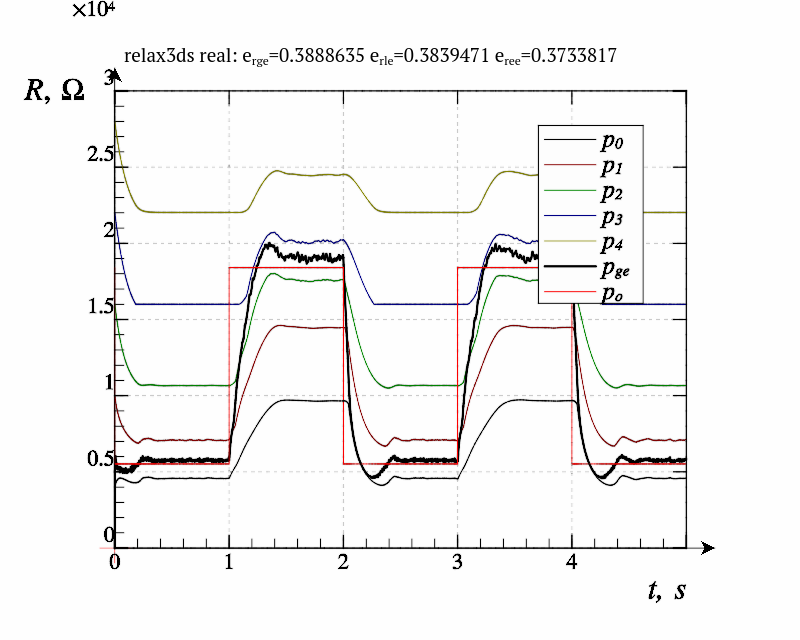
\includegraphics[width=0.45\textwidth]{p/relax3d_read_id2_3-p_p.png}
    \hfill
    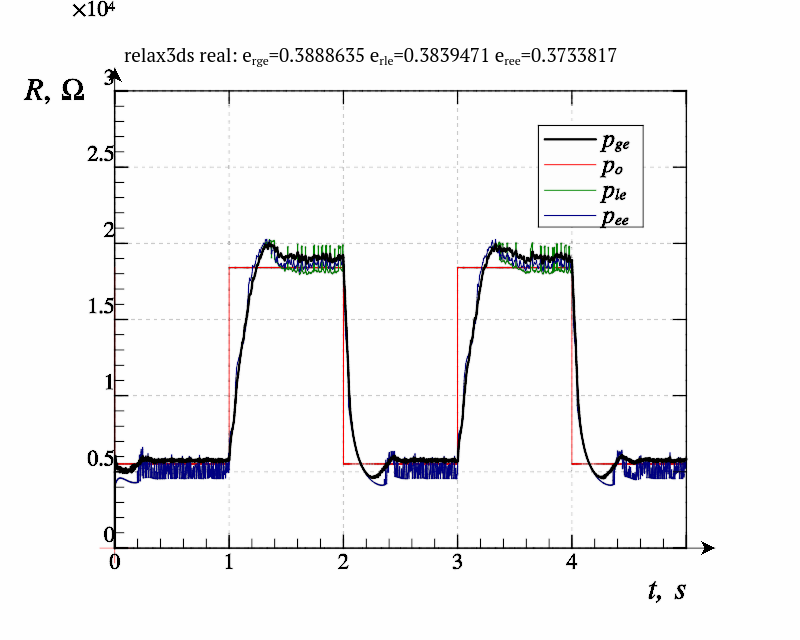
\includegraphics[width=0.45\textwidth]{p/relax3d_read_id2_3-p_pp.png}
  }
  \caption{Идентификация 3ds 3}
  \label{atu:f:relax3ds_id_3}
\end{figure}

\section{Выводы по разделу \thechapter}

Выводы.


